\chapter{Metoda voditeljev}

Velika prednost metode hierarhičnega gručenja, ki smo jo spoznali v prejšnjem poglavju, je odkrivanje strukture skupin v podatkih, ki jih lahko enostavno ponazorimo v vizualizaciji imenovani dendrogram. Na podlagi te vizualizacije lahko potem (intuitivno) presojamo o kvaliteti gručenja ter se odločamo o tem, na koliko skupin bomo razbili podatke. Zanimiva je tudi uporaba te tehnike pri interaktivni analizi podatkov v orodjih, ki nam take vizualizacije ponujajo in kjer lahko gradimo delokroge \angl{workflows}, s katerimi lahko izbrane skupine nadalje opišemo in interpretiramo.

A pri tem naletimo na največjo pomankljivost hierarhičnega gručenja: metoda deluje samo na relativno majhnih množicah podatkov. Če imamo podatkov veliko, recimo nekaj deset tisoč ali pa celo milijon, hierarhično gručenje zaradi časovne in prostorske kompleksnosti odpove, dendrogram pa postane prevelik in neuporaben.

Rešitev, ki dobro deluje na velikih množicah podatkov je postopek, ki ga imenujemo metoda voditeljev \angl{$K$-means}. Seveda zastonj kosila tudi tu ni. V svoji
osnovni inačici metoda voditeljev predpostavlja, da je uporabnik v naprej določil število skupin,
na katero želi razbiti učno množico primerov. Algoritem uporablja
t.im. voditelje oziroma primere, ki določajo te skupine oziroma so
središča skupin. Postopek iskanja optimalnega razbitja je potem
naslednji:

\begin{itemize}
\item prični s $K$ naključno izbranimi voditelji $\mathcal{V}=\{v^{(i)};\ i\in{1\ldots K}\}$
\item {\bf ponavljaj}
\begin{itemize}
  \item določi razvrstitev $\mathcal{C}$ tako, da vsak primer prirediš
    najbližjemu voditelju
  \item novi voditelji naj bodo centroidi $R(C_i)$ skupin $C_i\in\mathcal{C}$, $v^{(i)}\leftarrow R(C_i)$
\end{itemize}
\item {\bf dokler} se lega voditeljev spreminja
\end{itemize}

Voditelji \angl{centroids} so navadno kar geometrijska središča primerov skupine:

$$ R(C_i) = {1\over |C_i|} \sum_{x\in C_i}x $$

Izračun teh je za zvezne atribute preprost. Ker moramo v vsaki iteraciji izračunati razdaljo do $K$ voditeljev, je časovna kompleksnost tega algoritma le linearno odvisna od števila primerov, to je $O(I*k*m)$, kjer je $I$ število iteracij. Algoritem tipično hitro konvergira h končni rešitvi. Za srednje velike probleme (npr. nekaj 1000 primerov) je lahko potrebnih manj kot 100 iteracij.

Potek optimizacije za podatke, ki so bili opisani z dvema zveznima atributoma in so vključevali 780 primerov, je prikazan na sliki~\ref{f-kmeans-trace}. Za prikazano optimizacijo je zanimivo tudi število primerov, ki so pri posameznih iteracijah spremenili svojega voditelja:
%
\begin{verbatim}
Iteration: 1, changes: 54
Iteration: 2, changes: 21
Iteration: 3, changes: 18
Iteration: 4, changes: 18
Iteration: 5, changes: 18
Iteration: 6, changes: 29
Iteration: 7, changes: 63
Iteration: 8, changes: 131
Iteration: 9, changes: 64
Iteration: 10, changes: 6
Iteration: 11, changes: 0
\end{verbatim}
%
Optimizacija se skoraj ulovi v lokalni minimum, potem pa se v osmi
iteraciji pobere in poišče rešitev, ki se nam v tem primeru zdi smiselna.

\begin{figure}[htbp]
\begin{center}
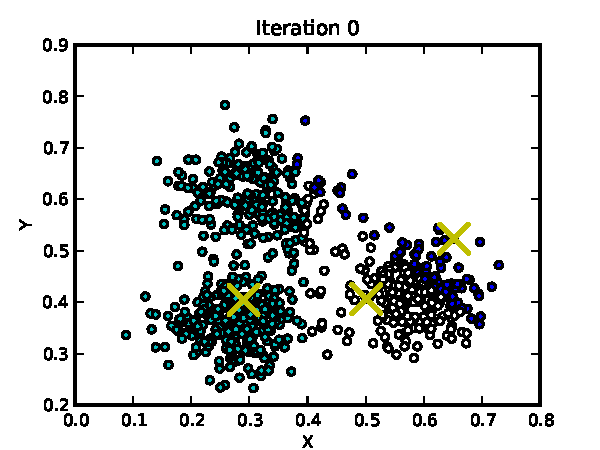
\includegraphics[width=5cm]{slike/kmeans-scatter-000.pdf}
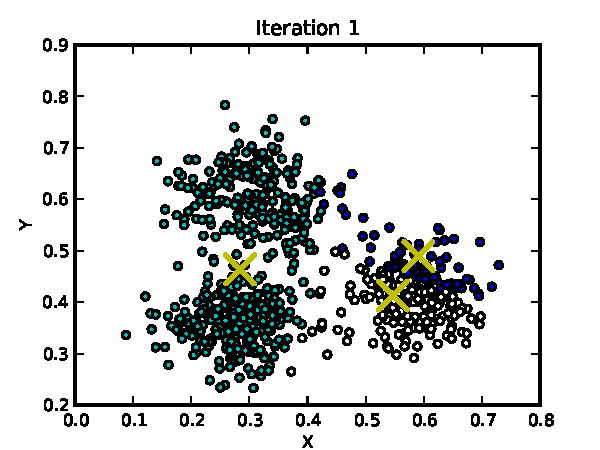
\includegraphics[width=5cm]{slike/kmeans-scatter-001.pdf}
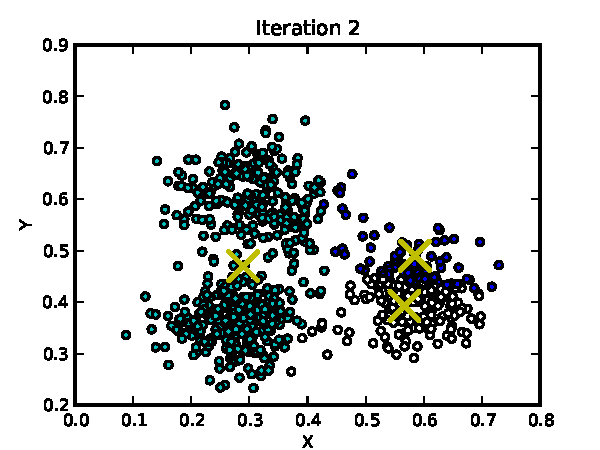
\includegraphics[width=5cm]{slike/kmeans-scatter-002.pdf}
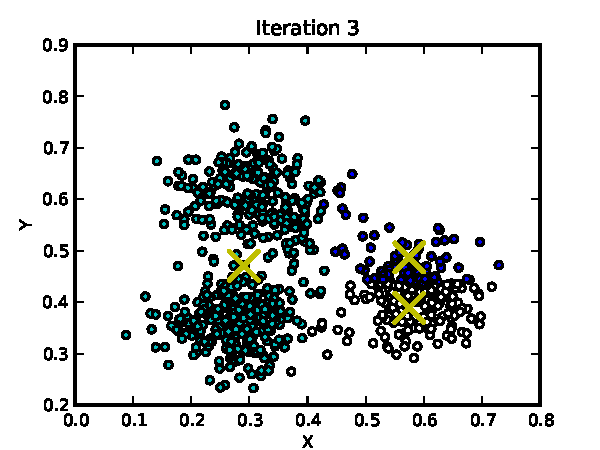
\includegraphics[width=5cm]{slike/kmeans-scatter-003.pdf}
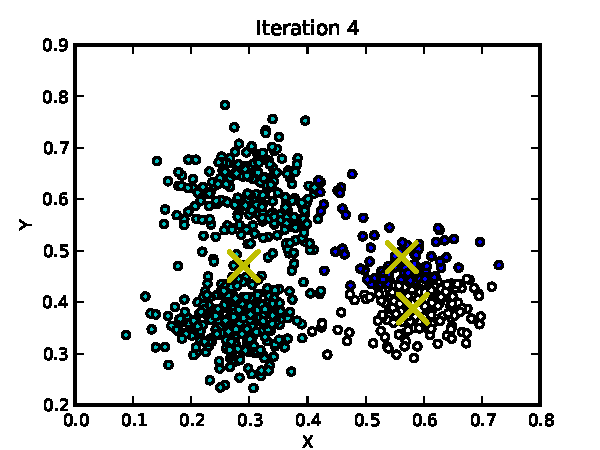
\includegraphics[width=5cm]{slike/kmeans-scatter-004.pdf}
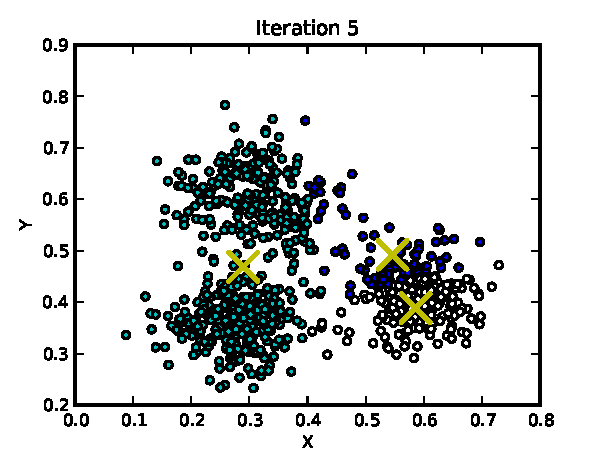
\includegraphics[width=5cm]{slike/kmeans-scatter-005.pdf}
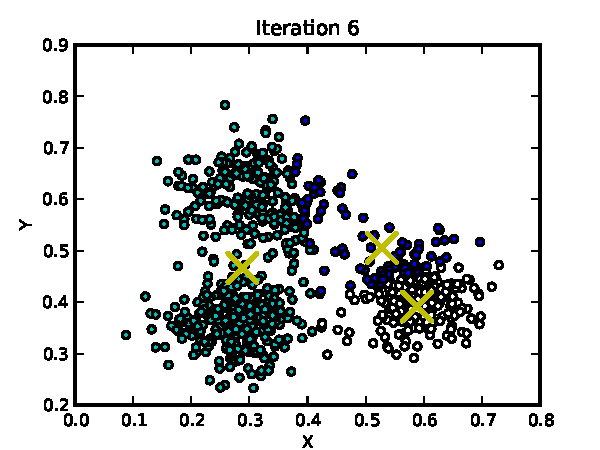
\includegraphics[width=5cm]{slike/kmeans-scatter-006.pdf}
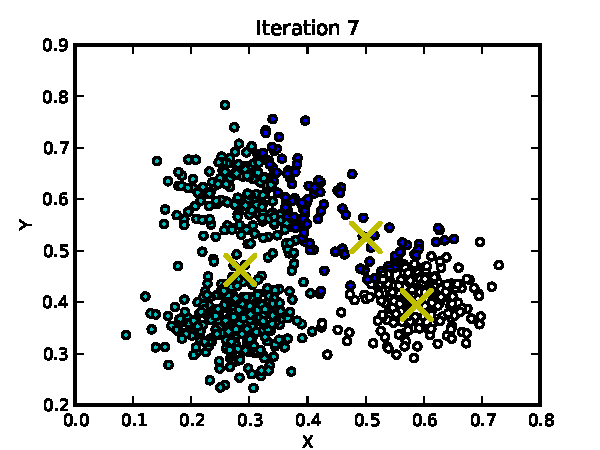
\includegraphics[width=5cm]{slike/kmeans-scatter-007.pdf}
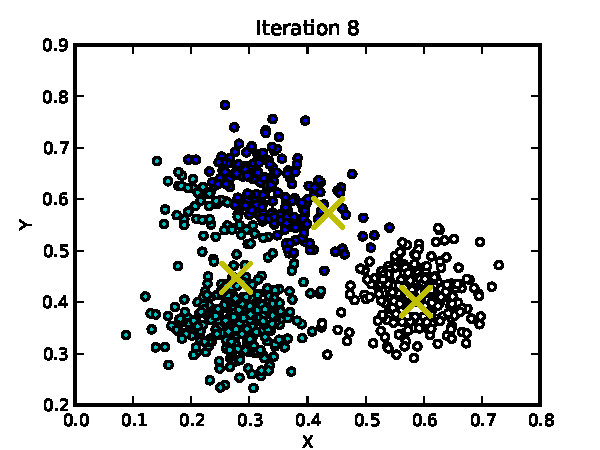
\includegraphics[width=5cm]{slike/kmeans-scatter-008.pdf}
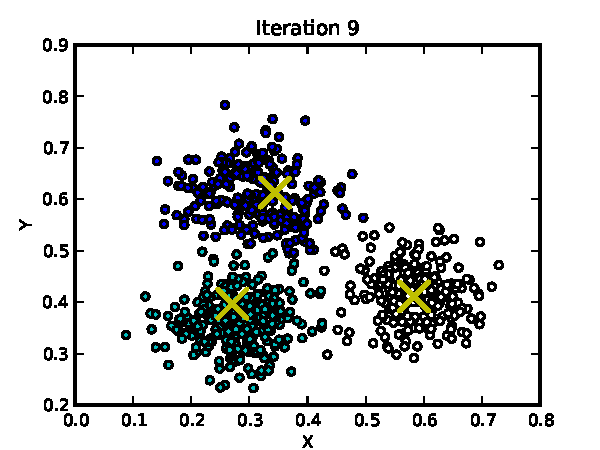
\includegraphics[width=5cm]{slike/kmeans-scatter-009.pdf}
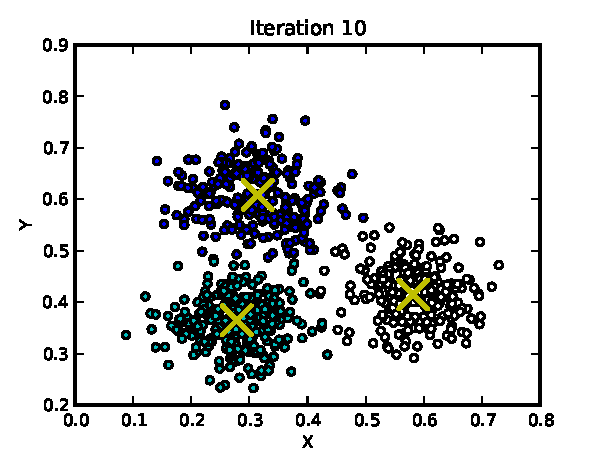
\includegraphics[width=5cm]{slike/kmeans-scatter-010.pdf}
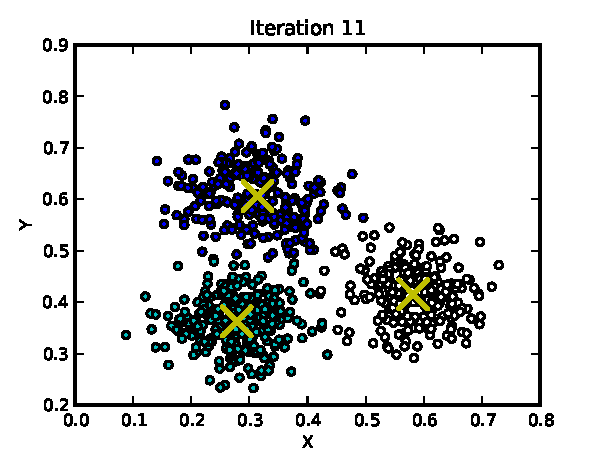
\includegraphics[width=5cm]{slike/kmeans-scatter-011.pdf}
\caption{Potek optimizacije razbitja za 780 primerov v evklidski
  ravnini. Lega voditeljev je označena s križcem. Primeri, ki
  pripadajo istemu voditelju, so označeni z isto barvo.}
\label{f-kmeans-trace}
\end{center}
\end{figure}

Tehnika voditeljev pa nas, za izbrane podatke in parametre metode,
lahko tudi preseneti in vrne nepričakovane rezultate. Primer take
razvrstitve je prikazan na sliki~\ref{f-kmeans-stripes}.

\begin{figure}[htbp]
\begin{center}
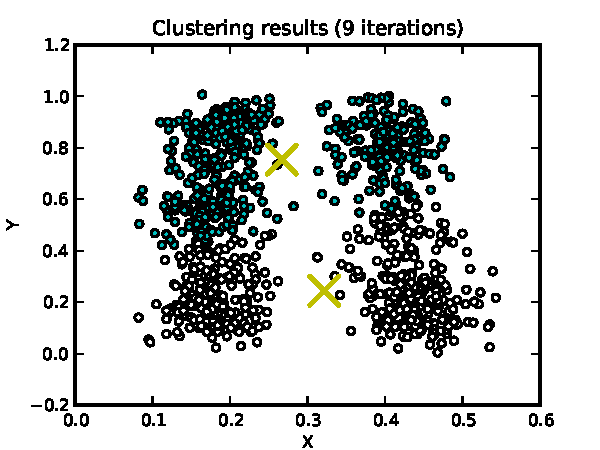
\includegraphics[width=8cm]{slike/kmeans-stripes.pdf}
\caption{Na pogled nepravilno razbitje, ki ga je predlagala metoda voditeljev.}
\label{f-kmeans-stripes}
\end{center}
\end{figure}

Rezultati metode voditeljev so lahko zelo občutljivi na izbor
primernih začetnih pogojev in mero razdalje med primeri (pri zgornjih
primerih smo uporabljali evklidsko razdaljo).

\subsection{Začetni izbor voditeljev}

Razbitje, ki ga vrne metoda voditeljev, je lahko zelo odvisna od
začetnega izbora voditeljev. Od te bo tudi odvisno število iteracij,
ki so potrebne, da postopek privedejo v stabilno stanje, v katerem so
izpolnjeni ustavitveni pogoji. Zato je smiseln študij tehnik, ki bi
voditelje izbrala čim bolje. Znanih je nekaj standardnih prijemov:

\begin{description}
\item[Naključni izbor voditeljev.] Za tega smo sicer že povedali, da
  lahko privede v neoptimalno razbitje. A se lahko temu izognemo, če
  postopek ponovimo večkrat in med poiskanimi razbitji izberemo
  najboljše. \comment{Kako to storimo? Katero razbitje je najboljše?}
\item[Izbor razpršenih voditeljev.] Poiščemo primer, ki je najbolj
  oddaljen od drugih. Naj bo to naš prvi voditelj. Potem poiščemo
  primer, ki je njemu najbolj oddaljen. To je drugi
  voditelj. Naslednje voditelje poiščemo tako, da so ti najbolj
  oddaljeni od voditeljev, ki smo jih že določili.
\item[Uporaba hierarhičnega razvrščanja.] Na podmnožici točk s
  hierarhičnim razvrščanjem poiščemo $K$ skupin in njihova
  središča uporabimo kot začetne voditelje. \comment{Zakaj ne
    uporabimo celotnega nabora primerov?}
\end{description}

\subsection{Ustavitveni kriterij}

V osnovnem algoritmu za iskanje razbitij po metodi voditeljev
zahtevamo, da se postopek ustavi šele takrat, ko se razbitje več ne
spreminja. Takrat noben primer ne zamenja svojega centroida. V
splošnem temu pogoju ne moremo vedno zadostiti, saj se nam lahko
zgodi, da pride do oscilacij in se postopek na omenjeni način nikoli
ne zaustavi. A so ti primeri v praksi zelo redki. Pri velikih množicah
primerov, in v izogib nestabilnosti, lahko namesto popolne stabilnosti
rešitve postopka zahtevamo, da se ta izteče, ko v iteraciji samo nekaj
(na primer 10) primerov ali manj zamenja skupino.

\subsection{Ocenjevanje kvalitete razbitij}

Glavna pomanjkljivost metode voditeljev, tudi z ozirom na tehniko
hierarhičnega razvrščanja v skupine, je potreba po izboru števila
skupin $K$. Uporabnik le redkokdaj ve, na koliko skupin bi bilo
potrebno rezultate razbiti. Pravzaprav je prav ``pravo'' število
skupin ena od ključnih informacij, ki bi jih radi na podlagi podatkov
ocenili.

Tu se zatečemo k razmisleku o cilju razbitja podatkov na skupine. V
splošnem bi želeli poiskati taka razbitja, kjer so si primeri znotraj
skupine čim bolj podobni, ter primeri iz različnih skupin čim bolj
različni. Če razmišljamo samo o prvem, potem želimo, da metoda
voditeljev poišče tako razbitje, kjer bo vsota oddaljenosti od
pripadajočih voditeljev oziroma spodnji izraz čim manjši:
%
$$ \sum_{i=1}^K \sum_{x\in Ci} d(m^{(i)}, x) $$
%
Predpostavimo, da se naši primeri nahajajo v evklidski ravnini in da imamo opravka s podatki z enim samim atributom. Razdaljo med točkami bomo merili z evklidsko razdaljo. Zgornji izraz se prevede v vsoto kvadratnih napak \angl{sum of squared errors, SSE} oziroma odstopanj od centroidov:
%
$$SSE = \sum_{i=1}^K \sum_{x\in Ci}(m^{(i)}-x)^2$$
%
Iščemo take centroide $C_k$, kjer je ta napaka najmanjša:
\begin{eqnarray}
\pd{}{m^{(k)}} & = & \pd{}{m^{(k)}}\sum_{i=1}^K\sum_{x\in C_i}(m^{(i)}-x)^2  \\
& = & \sum_{i=1}^K\sum_{x\in C_i} \pd{}{m^{(k)}}(m^{(i)}-x)^2 \\
& = & \sum_{x\in C_k} 2 (m^{(k)}-x)
\end{eqnarray}
%
\begin{equation}
\sum_{x\in C_k} 2 (m^{(k)}-x) = 0 \ \Rightarrow \ |C_k|\ m^{(k)} = \sum_{x\in C_k}
  x \ \Rightarrow \ m^{(k)} = {1 \over |C_k|} \sum_{x\in C_k}x
\end{equation}
%
kjer je $|C_k|$ število primerov v skupini $C_k$. Najboljši centroidi,
ki minimizirajo vsoto kvadratnih napak so ravno centri (središnjice)
skupin. Če bi vzeli namesto evklidske razdalje Manhattansko, bi s
pomočjo podobnega izvajanja kot zgoraj dobili, da so najbolj primerni
centri mediane točk v skupini.

Pri zgornjem izvajanju smo se osredotočili le na zmanjševanje
oddaljenosti točk v skupini od njihovih centroidov. Pravzaprav pa nas
zanima podobnost primerov znotraj skupine oziroma t.im. kohezija, ter
oddaljenost primerov med različnimi skupinami, oziroma
t.im. ločljivost. Mera kvalitete razbitja, ki uspešno združuje tako
kohezijo kot ločljivost je silhuetni koeficient, oziroma silhueta
razbitja. Izračunamo ga s sledečim postopkom:
\begin{itemize}
\item Naj bo $a_i$ povprečna razdalja primera $x^{(i)}$ do vseh ostalih primerov v njegovi skupini.
\item Za primer $x^{(i)}$ in neko skupino $C_j;\ x_i\not\in C_j$, ki   je različna od te, ki vsebuje $x_i$, izračunaj povprečno razdaljo   med $x_i$ in primeri v tej skupini. Poišči skupino $C_j$, kjer je ta   razdalja najmanjša. Imenujmo to razdaljo $b_i$.
\item Za primer $x_i$ je njegova silhueta enaka
  $s_i=(b_i-a_i)/\max(a_i,b_i)$.
\item Silhueta razbitja je enaka povprečni silhueti primerov v učni
  množici:
$$s={1 \over |\mathcal{U}|}\sum_{i=1}^{|\mathcal{U}|} s_i$$
\end{itemize}

Možne vrednosti silhuetnega koeficienta v teoriji ležijo na intervalu
med -1 do 1, v praksi pa pričakujemo, da bo za dani primer razdalja do
primerov v lastni skupini veliko manjša od razdalj do primerov v
najbližji tuji skupini, torej $a_i<b_i$ in zato $s_i>0$. V primeru, ko
so te razlike velike, je vrednost silhuete 1. Silhuete primerov lahko
izrišemo za vsako skupino. Uredimo jih od največjega do najmanjšega
(za primer, kjer smo razvrstili podatke nabora ``voting'' v tri
skupine, glej sliko~\ref{f-kmeans-silhouette-voting}). Kateri primeri so tisti, ki imajo kratko silhueto?

\begin{figure}[htbp]
\begin{center}
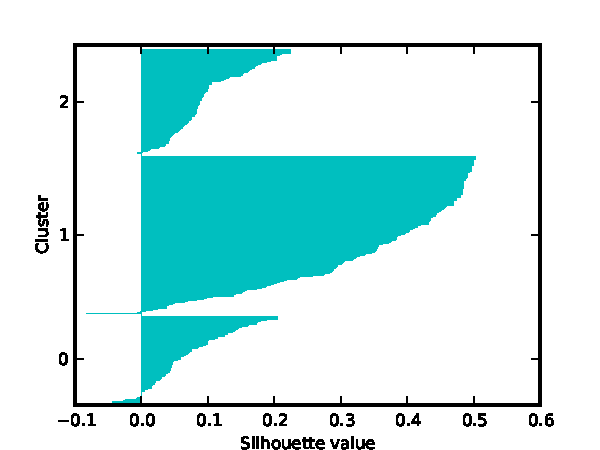
\includegraphics[width=10cm]{slike/kmeans-silhouette-voting.pdf}
\caption{Silhuete primerov iz podatkovnega nabora ``voting'' pri
  razvrstitvi v tri skupine.}
\label{f-kmeans-silhouette-voting}
\end{center}
\end{figure}

Kvaliteto razbitja za dano število skupin $K$ lahko torej ocenimo s
povprečno silhueto primerov. To nam omogoča, da ocenimo, kako primerne
so različne vrednosti $K$ (glej primer take študije s
slike~\ref{f-kmeans-silhouette-study}). Hevristika sicer ne deluje
idealno, a nam lahko, z malce previdnosti, pomaga, da izberemo
primerno število skupin za naše podatke. Previdnost je potrebna
predvsem tam, kjer so razlike med silhuetami majhne. V takih primerih
nam pomaga razmišljanje o tem, kaj posamezne skupine sploh sestavlja
in kakšne so skupne značilnosti primerov v skupinah.

\begin{figure}[htbp]
\begin{center}
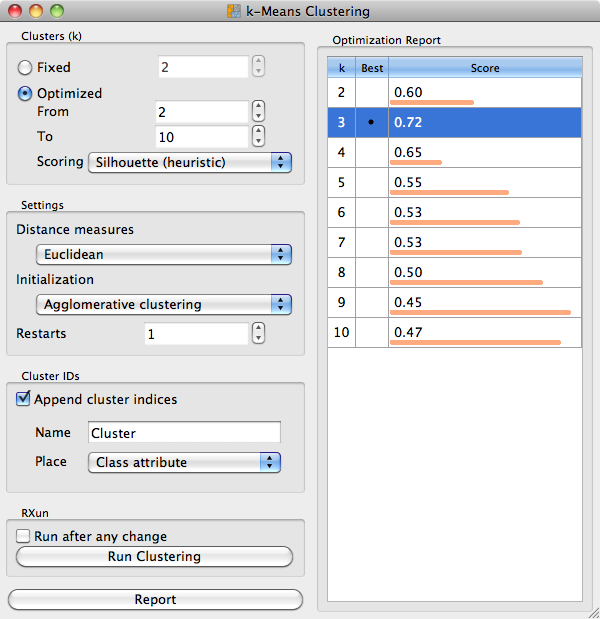
\includegraphics[width=10cm]{slike/kmeans-silhouette-study.png}
\caption{Silhuetna študija razvrstitve v različno število skupin za
  podatke s slike~\ref{f-kmeans-trace}.}
\label{f-kmeans-silhouette-study}
\end{center}
\end{figure}

\section{Kombiniranje razvrstitev in razvrščanje s konsenzom}

``Več ljudi več ve'', ali modrost množic. Tudi na področju razvrščanja
je lahko tako. Različni algoritmi, njihovi parametri ali pa rahlo
različne učne množice iz iste problemske domene nam lahko pomagajo
razkriti skupine, ki so lahko rahlo, ali pa tudi precej različne med
sabo. Bi bilo pametno, pri takem nizu razvrstitev, te skupine nekako
zliti in poiskati stabilni del razvrstitev. Če bi na primer dva
primera pri večini razvrstitev bila del istih skupin bi to bil dober
pokazatelj, da bi bilo dobro ta dva primera tudi sicer razvrstiti
skupaj. Po drugi strani pa bi lahko za dva druga primera, ki ju skoraj
nikoli nismo našli v skupnih skupinah, rekli, da pač ne sodita skupaj.

Na zgornji ideji temelji algoritem razvrščanja s
konsenzom (Monti in sod., 2003), ki ga opišemo s spodnjim algoritmom.
% \cite

\begin{tabbing}
xxx\=xxx\=xxxxxxxxxxxxxxxxxxxxxxxxxxxxxxxxxxxxxxx\=\kill
{\bf input:} \\
\> učna množica primerov $D$ \\
\> algoritem razvrščanja Cluster in izbrano število skupin $K$ \\
\> število vzorčenj $H$ \\
\\
$M\Leftarrow\emptyset$ \>\>\> množica povezovalnih matrik\\
{\bf for} $h=1,2,\ldots, H$ {\bf do} \\
\> $D^{(h)}\leftarrow {\rm Resample}(D)$ \>\> izberemo vzorec iz
učne množice \\
\> $M^{(h)}\leftarrow {\rm Cluster}(D^{(h)}, K)$ \>\> razvrstimo
primere iz $D^{(h)}$ v $K$ skupin \\
\> $M\leftarrow M\cup M^{(h)}$ \\
{\bf end} \\
$\mathcal{M}\leftarrow$ ComputeConsensusMatrix$(M)$ \\
$\mathcal{C}\leftarrow$ razbitje $D$ v $K$ skupin na podlagi $\mathcal{M}$
\end{tabbing}

Oznaka $M^{(h)}$ označuje povezovalno matriko:
$$ M^{(h)}(i,j) = \left\{
     \begin{array}{ll}
       1 & = X_i\in C\wedge X_j\in C \\
       0 & = \text{otherwise}
     \end{array}
   \right.$$
Iz množice povezovalnih matrik izračunamo matriko konsenzov:
$$ \mathcal{M}(i,j) = {\sum_h M^{(h)}(i,j) \over \sum_h
  I^{(h)}(i,j)} $$
Kjer je $I$ matrika indikatorjev, ki ima za par $i$ in $j$ vrednost 1,
če sta oba primera $X_i$ in $X_j$ prisotna v vzorcu $D^{(h)}$, sicer
pa vrednost 0. Elementi povezovalne matrike so realna števila na
intervalu od 0 do 1. Elementi ustrezajo podobnostim primerov, matrika
pa podobnostni matriki. Matrika ${\bf 1}-\mathcal{M}$ je zato matrika
razdalj med primeri, ki jo lahko uporabimo pri hierarhičnem
razvrščanju v primere ter na ta način pridobimo možne razvrstitve, ki
predstavljajo konsenz delnih razvrstitev na vzorcih iz učne množice.

\subsection{Permutacijski test}

Včasih nam tudi kvantitativna ocena, kot je silhueta, neposredno ne
pove prav dosti o tem, ali so v podatkih zares skupine ali pa je
algoritem našel neko razbitje, ki pa bi bilo podobne kvalitete tudi,
če bi bili podatki naključni oziroma, bolje, taki, kjer bi sicer
ohranili porazdelitve vrednosti posameznih atributov a izničili
interakcije med atributi. V nadaljevanju bomo zaradi poenostavitve
take podatke imenovali naključni podatki.

\begin{figure}[htbp]
\begin{center}
  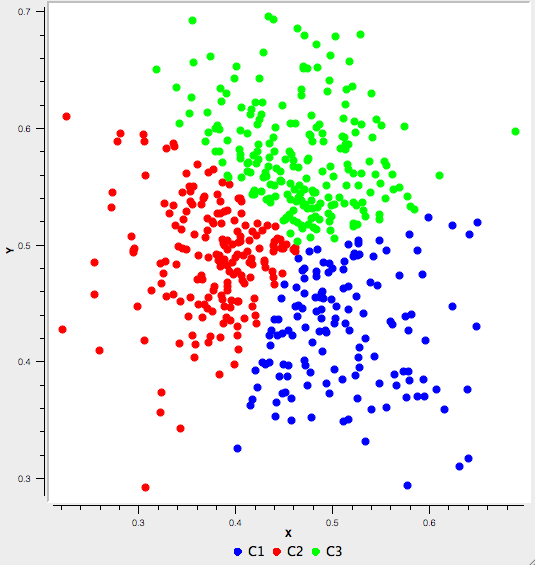
\includegraphics[width=6cm]{slike/kmeans-wrong-scatter.png}
\caption{Rezultat razbitja s tehniko voditeljev na dvoatributni domeni
izgleda lepo strukturiran, vprašanje pa je, ali smo res odkrili tri
značilne skupine. Silhueta tega razbitja je $0.50$ in je bila le rahlo
različna od silhuete za ostala razbitja na dve do deset skupin, kjer
je bila silhueta od $0.44$ do $0.49$.}
\label{f-kmeans-hairball}
\end{center}
\end{figure}


Naša hipoteza, ki jo preizkušamo in jo v statistiki imenujemo ničelna
hipoteza, je ($H_0$): silhueta $s$ ima vrednost, kot bi jo dobili,
če bi bili podatki naključni.

Zgornjo hipotezo je enostavno računsko preveriti. Generirajmo naključne
podatke. To storimo tako, da v naših podatkih za vsak atribut
naključno premešamo njihove vrednosti po primerih. Ker so podatki
podani v tabeli, je to isto, kot če vrednosti vsake kolone med sabo
premešamo. (Je to res potrebno narediti za vse kolone oziroma
atribute?) Na teh podatkih uporabimo tehniko razvrščanja in izmerimo
silhueto. To ponovimo, na primer vsaj 100-krat ali pa bolje
1000-krat. Na ta način dobimo porazdelitev vrednosti naše statistike
$s$, kot bi jo dobili, če bi ta izhajala iz naključnih
podatkov. Izmerimo sedaj to isto statistiko na nepremešanih,
originalnih podatkih in jo primerjamo z ničelno porazdelitvijo.

Zgornji postopek smo uporabili na podatkih, ki so bili podobni tem iz
slike~\ref{f-kmeans-hairball}. Za oceno ničelne porazdelitve smo
izračunali $200$ silhuet, vsakič na podatkih s premešanimi vrednostmi
atributov. Ugotovimo, da je kar $23\%$ vseh vrednosti iz ničelne
distribucije večje od naše opazovane statistike na originalnih
podatkih. Če bi trdili, da je naša ničelna hipoteza $H_0$ napačna, bi
na podlagi naših eksperimentov verjetnost napačne zavrnitve te
hipoteze bila $p=0.23$. V statistiki je to veliko prevelik prag za
zavrnitev ničelne hipoteze. Tipično je sprejemljiva meja tega praga
enaka $\alpha=0.01$, včasih celo $\alpha=0.05$. 

\begin{figure}[htbp]
\begin{center}
  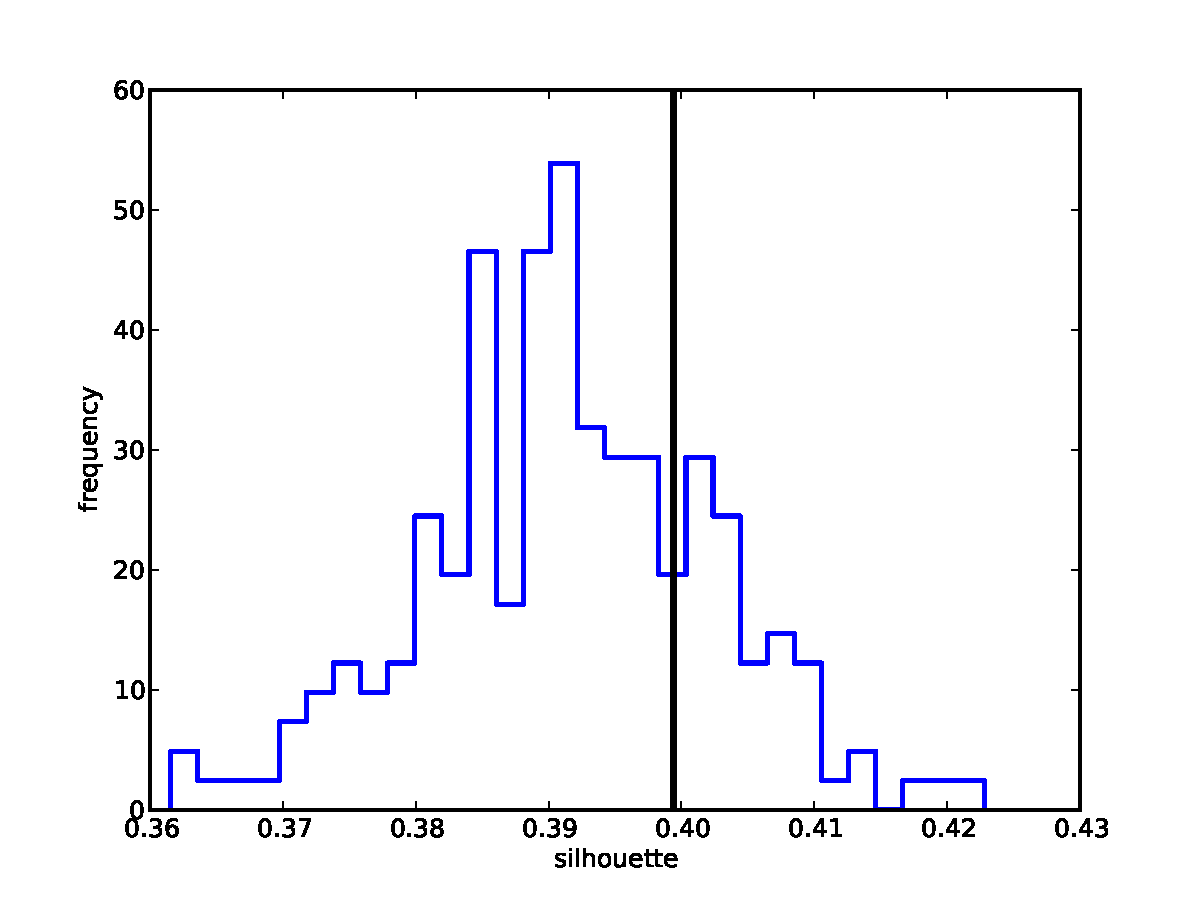
\includegraphics[width=10cm]{slike/kmeans-permutations.pdf}
\caption{Porazdelitev silhuet na permutiranih podatkih in projekcija
  (ravna črta) silhuete na originalnih podatkih kaže na to, da, vsaj
  za izbrano število skupin, za te podatke nismo našli smiselnega razbitja.}
\label{f-kmeans-permutations}
\end{center}
\end{figure}

Za konec si poglejmo še malce drugačne podatke
(slika~\ref{f-kmeans-two-overlap}). Tu so rezultati smiselni oziroma
tako vsaj zgledajo. Podatki dejansko nakazujejo, da bi lahko imeli
dve skupini. To preverimo s permutacijskim testom
(slika~\ref{f-kmeans-permutations-two}). Ničelno hipotezo zavrnemo z
verjetnostjo, da smo se pri tem zmotili $p=0.025$.

\begin{figure}[htbp]
\begin{center}
  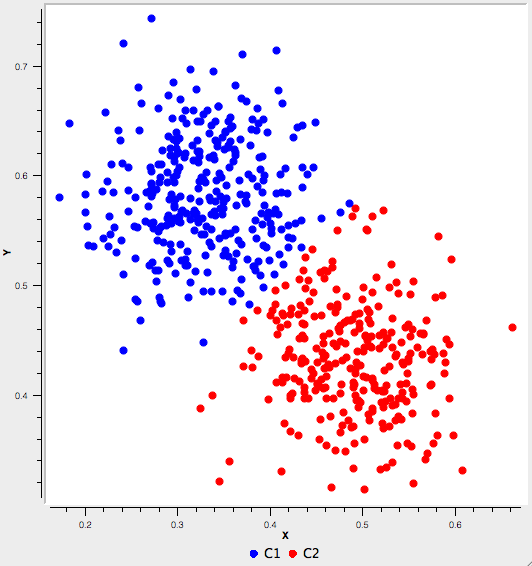
\includegraphics[width=6cm]{slike/kmeans-two-overlap.png}
\caption{Rezultat razbitja je tu morda smiseln. Silhueta za $K=2$ je
  0.68, za ostale vrednosti $K$ pa pod 0.56. Rezultate bi bilo dobro
  preveriti s permutacijskim testom.}
\label{f-kmeans-two-overlap}
\end{center}
\end{figure}

\begin{figure}[htbp]
\begin{center}
  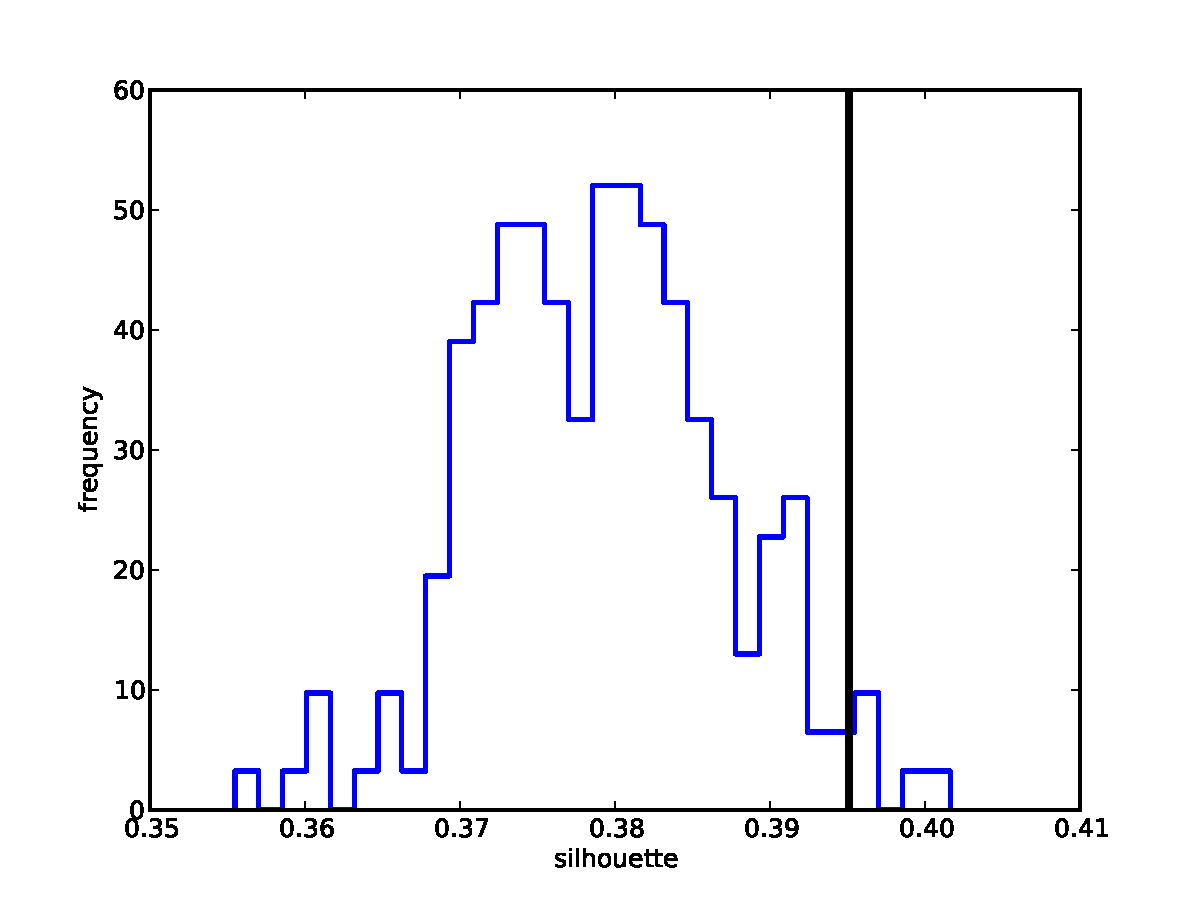
\includegraphics[width=10cm]{slike/kmeans-permutations-two.pdf}
\caption{Porazdelitev silhuet na permutiranih podatkih in projekcija
  (ravna črta) silhuete na originalnih podatkih s slike~\ref{f-kmeans-two-overlap}.}
\label{f-kmeans-permutations-two}
\end{center}
\end{figure}

\section{Predobdelava podatkov}

Do tu smo predpostavili, da imajo atributi v naši podatkovni množici
isto, zvezno, zalogo vrednosti. Taka lastnost podatkov je med temi, ki
jih uporabljamo pri reševanju praktičnih problemov, le redka. Navadno
z atributi zapišemo različne lastnosti primerov, ki nastopajo v
različnih merskih enotah. Na primer dolžina, teža, višina, ocena v
neki ocenjevalni lestvici, pa rezultati na različnih testih, in
podobno. Mere razdalje, kot je Evklidska, ne ločijo med različnimi
merskimi lestvicami, zato je potrebno podatke spremeniti tako, da bodo
vrednosti atributov med seboj primerljive. To storimo z
normalizacijo. In sicer, za vsak atribut $j$ določimo najprej njegovo
povprečno vrednost:
%
$$ \mu_j=E[X_j]={1\over N}\sum_{i=1}^N X_{ij}$$
%
kjer je $X_{ij}$ vrednost $j$-tega atributa za $i$-ti primer. Podobno
določimo tudi standardni odklon atributa:
%
$$ \sigma_j=\sqrt{E[(X_j-\mu_j)^2]}=\sqrt{{1\over N} \sum_{i=1}^N
  (X_{ij}-\mu_j)^2}$$
Podatke zdaj normaliziramo tako, da so nove vrednosti v tabeli
podatkov $Z_{ij}$ enake:
$$ Z_{ij}={X_{ij}-\mu_j\over\sigma_j} $$
